\section{Aplikasi yang dibutuhkan}
Memerlukan XAMPP untuk instalasi Framework Phalcon.
\begin{itemize}
 \item Step 1: Download Install lah file DLL (Dynamic Link Library) Phalcon di link https://phalconphp.com/en/download, sesuaikan file dll nya dengan konfigurasi versi XAMPP Anda.
 \item Step 2: Extract phalcon-php.dll file ke direktori /php/ext di folder XAMPP.
 \end{itemize}
 \begin{figure}[h!]
\centerline{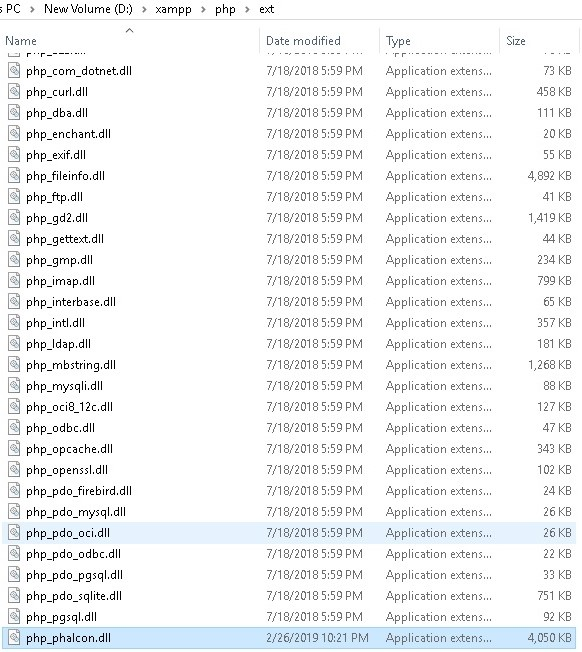
\includegraphics[width=0.5\textwidth]
{figures/directory.JPG}}
\caption{Masukkan file extension-nya disini}
\label{fig:directory}
\end{figure}
\begin{itemize}
 \item Step 3: Edit file php.ini didalam folder /XAMPP/php/php.ini. Tambahkan "extension=php\_phalcon.dll" tanpa tanda kutip ke baris akhir php.ini. Sesuai dengan gambar ~\ref{fig:extension}
\end{itemize}
\begin{figure}[h!]
\centerline{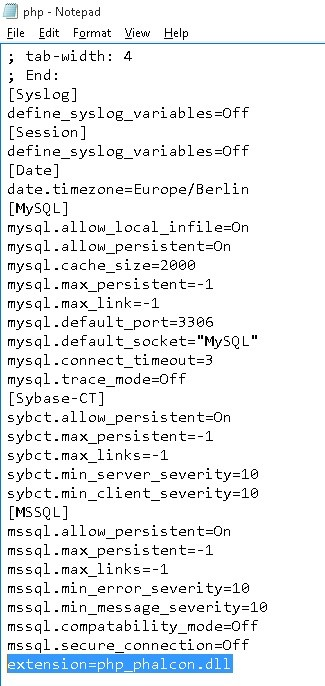
\includegraphics[width=0.5\textwidth]
{figures/extension.JPG}}
\caption{Apa yang harus di-edit di file php.ini}
\label{fig:extension}
\end{figure}
\begin{itemize}
 \item Step 4: Setelah itu, cek di localhost/dashboard/phpinfo.php, akan terdaftar library phalcon disana.
\end{itemize}
\begin{figure}[h!]
\centerline{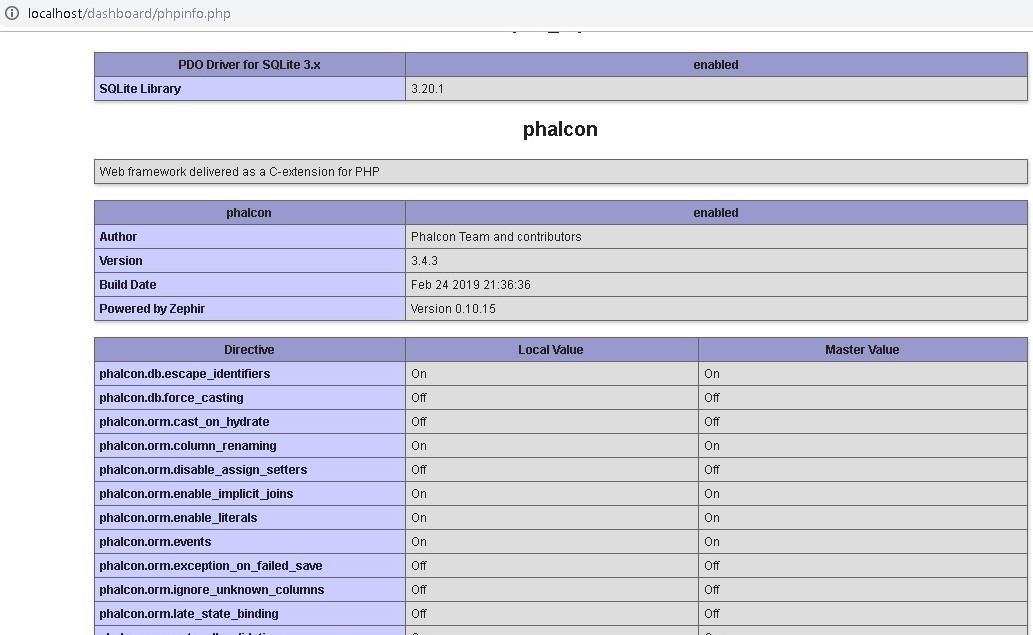
\includegraphics[width=0.5\textwidth]
{figures/phpinfo.JPG}}
\caption{Jika berhasil memasukkan ekstensi phalcon-nya}
\label{fig:phpinfo}
\end{figure}
\begin{itemize}
 \item Step 5: Install devtools master di situs https://github.com/phalcon/phalcon-devtools, simpan di direktori C, lalu Set Path Variable nya dengan menekan windows+R di keyboard, lalu ketikkan "sysdm.cpl SystemProperties" tanpa tanda kutip, masuk tab advance, lalu enviromental variables, klik new, dan masukkan path nya:
 \end{itemize}
\begin{figure}[h!]
\centerline{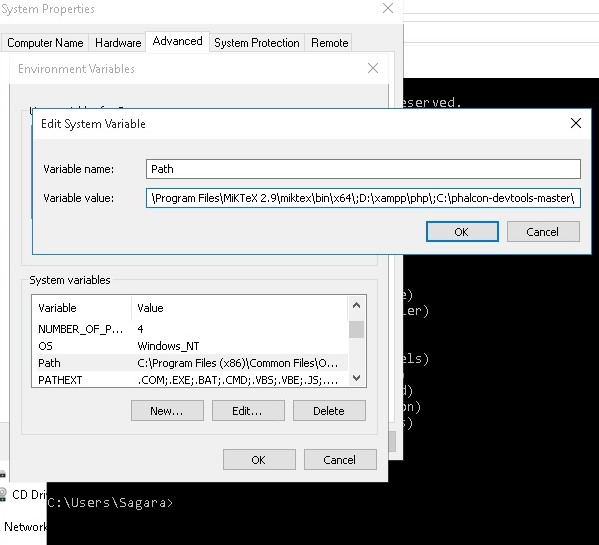
\includegraphics[width=0.5\textwidth]
{figures/variables.JPG}}
\caption{Masukkan path phalcon-devtools nya}
\label{fig:variables}
\end{figure}
\begin{itemize}
 \item Step 6: Path variable ini membantu Anda agar bisa menjalankan Phalcon Framework via cmd, terutama jika ingin membuat project yang baru:
  \end{itemize}
\begin{figure}[h!]
\centerline{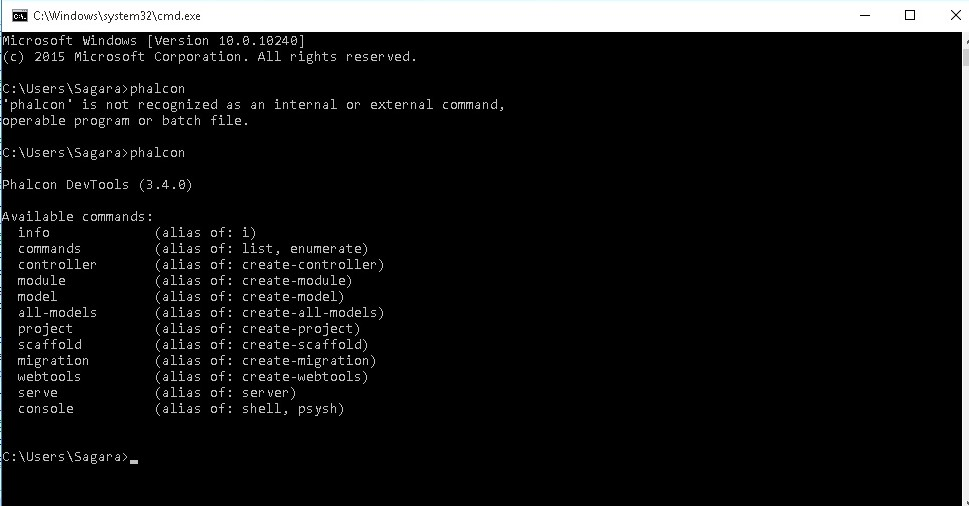
\includegraphics[width=0.5\textwidth]
{figures/test.JPG}}
\caption{Test di cmd apakah phalcon-devtools sudah terinstall atau belum}
\label{fig:test}
\end{figure}
\begin{itemize}
 \item Step 7: Setelah masuk cmd, ketikkan command seperti di ~\ref{lst:newproject}.
 \end{itemize}
\lstinputlisting[caption=Command untuk cara menambah project baru,label={lst:newproject}]{src/newproject.tex}
\begin{figure}[h!]
\centerline{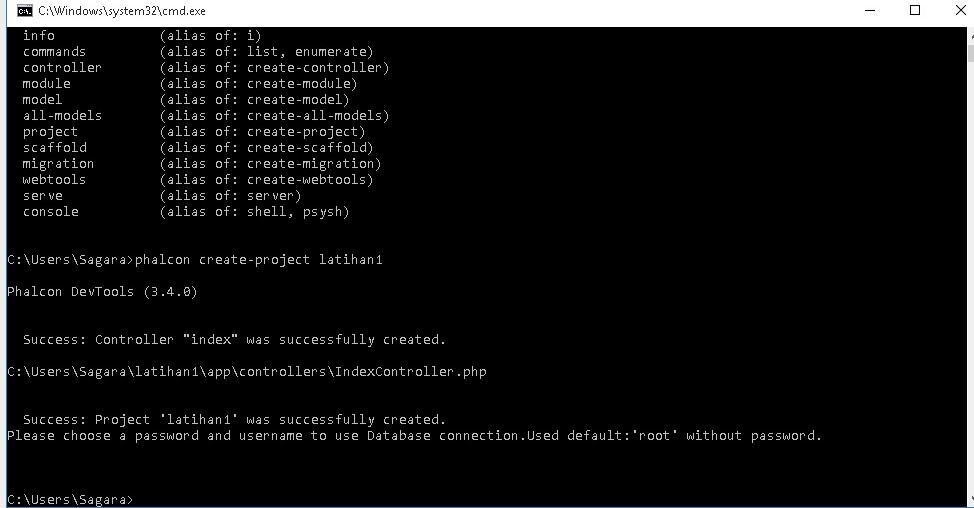
\includegraphics[width=0.5\textwidth]
{figures/newproject.JPG}}
\caption{Menambahkan Project Baru}
\label{fig:newproject}
\end{figure}
 \begin{itemize}
 \item Step 8: Project berhasil dibuat! masuk ke URL localhost/namaprojectanda
 \end{itemize}
 \begin{figure}[h!]
\centerline{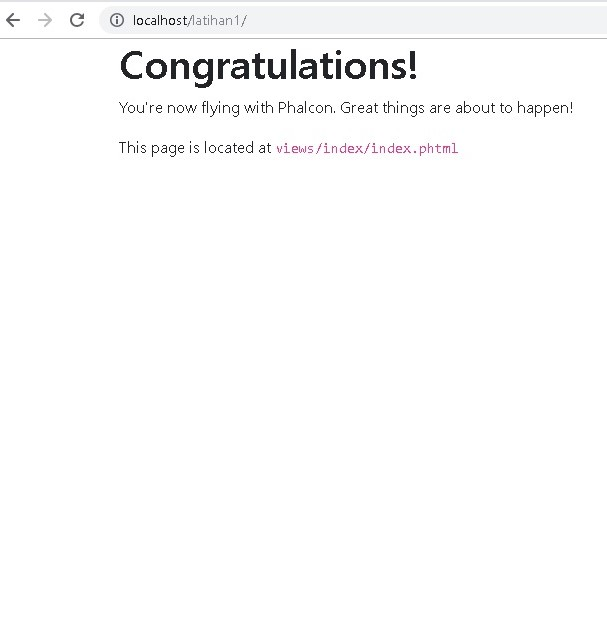
\includegraphics[width=0.5\textwidth]
{figures/hasil.JPG}}
\caption{Hasil new project}
\label{fig:hasil}
\end{figure}